\section{Sonnet: Nocturne}

\begin{figure}[h]\centering
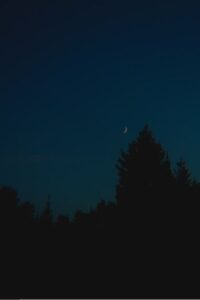
\includegraphics[width=.25\textwidth]{Nocturne-200x300.jpg}
\end{figure}

by \textbf{Mike M.}

\paragraph{Nocturne}

\begin{verse}
Crust covered, creaky feet, marching on twigs.\\ I gaze at the moon. Owls cry, none are seen.\\ Some stay `round the fire. Logs snap and scream.\\ I recall home, only the snout of pigs.

Seated, silent. All falls off in one glance.\\ Orion ambulates above. What can\\ I do with this life? Not one thing. What plan\\ Does man carry through infinite expanse?

Children joyfully toss `round the divine.\\ I join them knowing all the rules. Before\\ One mote of dust is the rose scent divine.

Rest now, your work boots have fallen apart.\\ You are never without. There is no lack.\\ Make it a comedy, make it your art.
\end{verse}

\flrightit{Posted on 2023-01-19 by Cologero}

\begin{center}* * *\end{center}

\begin{footnotesize}
\begin{sffamily}
\texttt{Naida on 2023-01-20 at 12:38 said:}

Beautiful!

\hfill

\texttt{Kaukomieli on 2023-01-21 at 06:56 said:}

This was enjoyable! Thank you.

I got so inspired that I wrote this just now.
\begin{verse}
I have carried the weight of Atlas\\ Upon my burderned shoulders\\ I discard the heavy baggage\\ Into the pit of wilderness

I am a dismal cry in the wilderness\\ Searching for the sacred centre\\ I am the cry of the white wolf\\ Holding up the banner of strength and wisdom

Alas, the Gods have now Fallen\\ And the Titans gain power\\ As caesarian rule destroys humanity

Where to look for salvation\\ now when everything\\ has crumbled to dust?
\end{verse}

\hfill

\end{sffamily}
\end{footnotesize}

